\documentclass{article} % For LaTeX2e
\usepackage{iclr2019_conference,times}

% Optional math commands from https://github.com/goodfeli/dlbook_notation.
%%%%% NEW MATH DEFINITIONS %%%%%

\usepackage{amsmath,amsfonts,bm}

% Mark sections of captions for referring to divisions of figures
\newcommand{\figleft}{{\em (Left)}}
\newcommand{\figcenter}{{\em (Center)}}
\newcommand{\figright}{{\em (Right)}}
\newcommand{\figtop}{{\em (Top)}}
\newcommand{\figbottom}{{\em (Bottom)}}
\newcommand{\captiona}{{\em (a)}}
\newcommand{\captionb}{{\em (b)}}
\newcommand{\captionc}{{\em (c)}}
\newcommand{\captiond}{{\em (d)}}

% Highlight a newly defined term
\newcommand{\newterm}[1]{{\bf #1}}


% Figure reference, lower-case.
\def\figref#1{figure~\ref{#1}}
% Figure reference, capital. For start of sentence
\def\Figref#1{Figure~\ref{#1}}
\def\twofigref#1#2{figures \ref{#1} and \ref{#2}}
\def\quadfigref#1#2#3#4{figures \ref{#1}, \ref{#2}, \ref{#3} and \ref{#4}}
% Section reference, lower-case.
\def\secref#1{section~\ref{#1}}
% Section reference, capital.
\def\Secref#1{Section~\ref{#1}}
% Reference to two sections.
\def\twosecrefs#1#2{sections \ref{#1} and \ref{#2}}
% Reference to three sections.
\def\secrefs#1#2#3{sections \ref{#1}, \ref{#2} and \ref{#3}}
% Reference to an equation, lower-case.
\def\eqref#1{equation~\ref{#1}}
% Reference to an equation, upper case
\def\Eqref#1{Equation~\ref{#1}}
% A raw reference to an equation---avoid using if possible
\def\plaineqref#1{\ref{#1}}
% Reference to a chapter, lower-case.
\def\chapref#1{chapter~\ref{#1}}
% Reference to an equation, upper case.
\def\Chapref#1{Chapter~\ref{#1}}
% Reference to a range of chapters
\def\rangechapref#1#2{chapters\ref{#1}--\ref{#2}}
% Reference to an algorithm, lower-case.
\def\algref#1{algorithm~\ref{#1}}
% Reference to an algorithm, upper case.
\def\Algref#1{Algorithm~\ref{#1}}
\def\twoalgref#1#2{algorithms \ref{#1} and \ref{#2}}
\def\Twoalgref#1#2{Algorithms \ref{#1} and \ref{#2}}
% Reference to a part, lower case
\def\partref#1{part~\ref{#1}}
% Reference to a part, upper case
\def\Partref#1{Part~\ref{#1}}
\def\twopartref#1#2{parts \ref{#1} and \ref{#2}}

\def\ceil#1{\lceil #1 \rceil}
\def\floor#1{\lfloor #1 \rfloor}
\def\1{\bm{1}}
\newcommand{\train}{\mathcal{D}}
\newcommand{\valid}{\mathcal{D_{\mathrm{valid}}}}
\newcommand{\test}{\mathcal{D_{\mathrm{test}}}}

\def\eps{{\epsilon}}


% Random variables
\def\reta{{\textnormal{$\eta$}}}
\def\ra{{\textnormal{a}}}
\def\rb{{\textnormal{b}}}
\def\rc{{\textnormal{c}}}
\def\rd{{\textnormal{d}}}
\def\re{{\textnormal{e}}}
\def\rf{{\textnormal{f}}}
\def\rg{{\textnormal{g}}}
\def\rh{{\textnormal{h}}}
\def\ri{{\textnormal{i}}}
\def\rj{{\textnormal{j}}}
\def\rk{{\textnormal{k}}}
\def\rl{{\textnormal{l}}}
% rm is already a command, just don't name any random variables m
\def\rn{{\textnormal{n}}}
\def\ro{{\textnormal{o}}}
\def\rp{{\textnormal{p}}}
\def\rq{{\textnormal{q}}}
\def\rr{{\textnormal{r}}}
\def\rs{{\textnormal{s}}}
\def\rt{{\textnormal{t}}}
\def\ru{{\textnormal{u}}}
\def\rv{{\textnormal{v}}}
\def\rw{{\textnormal{w}}}
\def\rx{{\textnormal{x}}}
\def\ry{{\textnormal{y}}}
\def\rz{{\textnormal{z}}}

% Random vectors
\def\rvepsilon{{\mathbf{\epsilon}}}
\def\rvtheta{{\mathbf{\theta}}}
\def\rva{{\mathbf{a}}}
\def\rvb{{\mathbf{b}}}
\def\rvc{{\mathbf{c}}}
\def\rvd{{\mathbf{d}}}
\def\rve{{\mathbf{e}}}
\def\rvf{{\mathbf{f}}}
\def\rvg{{\mathbf{g}}}
\def\rvh{{\mathbf{h}}}
\def\rvu{{\mathbf{i}}}
\def\rvj{{\mathbf{j}}}
\def\rvk{{\mathbf{k}}}
\def\rvl{{\mathbf{l}}}
\def\rvm{{\mathbf{m}}}
\def\rvn{{\mathbf{n}}}
\def\rvo{{\mathbf{o}}}
\def\rvp{{\mathbf{p}}}
\def\rvq{{\mathbf{q}}}
\def\rvr{{\mathbf{r}}}
\def\rvs{{\mathbf{s}}}
\def\rvt{{\mathbf{t}}}
\def\rvu{{\mathbf{u}}}
\def\rvv{{\mathbf{v}}}
\def\rvw{{\mathbf{w}}}
\def\rvx{{\mathbf{x}}}
\def\rvy{{\mathbf{y}}}
\def\rvz{{\mathbf{z}}}

% Elements of random vectors
\def\erva{{\textnormal{a}}}
\def\ervb{{\textnormal{b}}}
\def\ervc{{\textnormal{c}}}
\def\ervd{{\textnormal{d}}}
\def\erve{{\textnormal{e}}}
\def\ervf{{\textnormal{f}}}
\def\ervg{{\textnormal{g}}}
\def\ervh{{\textnormal{h}}}
\def\ervi{{\textnormal{i}}}
\def\ervj{{\textnormal{j}}}
\def\ervk{{\textnormal{k}}}
\def\ervl{{\textnormal{l}}}
\def\ervm{{\textnormal{m}}}
\def\ervn{{\textnormal{n}}}
\def\ervo{{\textnormal{o}}}
\def\ervp{{\textnormal{p}}}
\def\ervq{{\textnormal{q}}}
\def\ervr{{\textnormal{r}}}
\def\ervs{{\textnormal{s}}}
\def\ervt{{\textnormal{t}}}
\def\ervu{{\textnormal{u}}}
\def\ervv{{\textnormal{v}}}
\def\ervw{{\textnormal{w}}}
\def\ervx{{\textnormal{x}}}
\def\ervy{{\textnormal{y}}}
\def\ervz{{\textnormal{z}}}

% Random matrices
\def\rmA{{\mathbf{A}}}
\def\rmB{{\mathbf{B}}}
\def\rmC{{\mathbf{C}}}
\def\rmD{{\mathbf{D}}}
\def\rmE{{\mathbf{E}}}
\def\rmF{{\mathbf{F}}}
\def\rmG{{\mathbf{G}}}
\def\rmH{{\mathbf{H}}}
\def\rmI{{\mathbf{I}}}
\def\rmJ{{\mathbf{J}}}
\def\rmK{{\mathbf{K}}}
\def\rmL{{\mathbf{L}}}
\def\rmM{{\mathbf{M}}}
\def\rmN{{\mathbf{N}}}
\def\rmO{{\mathbf{O}}}
\def\rmP{{\mathbf{P}}}
\def\rmQ{{\mathbf{Q}}}
\def\rmR{{\mathbf{R}}}
\def\rmS{{\mathbf{S}}}
\def\rmT{{\mathbf{T}}}
\def\rmU{{\mathbf{U}}}
\def\rmV{{\mathbf{V}}}
\def\rmW{{\mathbf{W}}}
\def\rmX{{\mathbf{X}}}
\def\rmY{{\mathbf{Y}}}
\def\rmZ{{\mathbf{Z}}}

% Elements of random matrices
\def\ermA{{\textnormal{A}}}
\def\ermB{{\textnormal{B}}}
\def\ermC{{\textnormal{C}}}
\def\ermD{{\textnormal{D}}}
\def\ermE{{\textnormal{E}}}
\def\ermF{{\textnormal{F}}}
\def\ermG{{\textnormal{G}}}
\def\ermH{{\textnormal{H}}}
\def\ermI{{\textnormal{I}}}
\def\ermJ{{\textnormal{J}}}
\def\ermK{{\textnormal{K}}}
\def\ermL{{\textnormal{L}}}
\def\ermM{{\textnormal{M}}}
\def\ermN{{\textnormal{N}}}
\def\ermO{{\textnormal{O}}}
\def\ermP{{\textnormal{P}}}
\def\ermQ{{\textnormal{Q}}}
\def\ermR{{\textnormal{R}}}
\def\ermS{{\textnormal{S}}}
\def\ermT{{\textnormal{T}}}
\def\ermU{{\textnormal{U}}}
\def\ermV{{\textnormal{V}}}
\def\ermW{{\textnormal{W}}}
\def\ermX{{\textnormal{X}}}
\def\ermY{{\textnormal{Y}}}
\def\ermZ{{\textnormal{Z}}}

% Vectors
\def\vzero{{\bm{0}}}
\def\vone{{\bm{1}}}
\def\vmu{{\bm{\mu}}}
\def\vtheta{{\bm{\theta}}}
\def\va{{\bm{a}}}
\def\vb{{\bm{b}}}
\def\vc{{\bm{c}}}
\def\vd{{\bm{d}}}
\def\ve{{\bm{e}}}
\def\vf{{\bm{f}}}
\def\vg{{\bm{g}}}
\def\vh{{\bm{h}}}
\def\vi{{\bm{i}}}
\def\vj{{\bm{j}}}
\def\vk{{\bm{k}}}
\def\vl{{\bm{l}}}
\def\vm{{\bm{m}}}
\def\vn{{\bm{n}}}
\def\vo{{\bm{o}}}
\def\vp{{\bm{p}}}
\def\vq{{\bm{q}}}
\def\vr{{\bm{r}}}
\def\vs{{\bm{s}}}
\def\vt{{\bm{t}}}
\def\vu{{\bm{u}}}
\def\vv{{\bm{v}}}
\def\vw{{\bm{w}}}
\def\vx{{\bm{x}}}
\def\vy{{\bm{y}}}
\def\vz{{\bm{z}}}

% Elements of vectors
\def\evalpha{{\alpha}}
\def\evbeta{{\beta}}
\def\evepsilon{{\epsilon}}
\def\evlambda{{\lambda}}
\def\evomega{{\omega}}
\def\evmu{{\mu}}
\def\evpsi{{\psi}}
\def\evsigma{{\sigma}}
\def\evtheta{{\theta}}
\def\eva{{a}}
\def\evb{{b}}
\def\evc{{c}}
\def\evd{{d}}
\def\eve{{e}}
\def\evf{{f}}
\def\evg{{g}}
\def\evh{{h}}
\def\evi{{i}}
\def\evj{{j}}
\def\evk{{k}}
\def\evl{{l}}
\def\evm{{m}}
\def\evn{{n}}
\def\evo{{o}}
\def\evp{{p}}
\def\evq{{q}}
\def\evr{{r}}
\def\evs{{s}}
\def\evt{{t}}
\def\evu{{u}}
\def\evv{{v}}
\def\evw{{w}}
\def\evx{{x}}
\def\evy{{y}}
\def\evz{{z}}

% Matrix
\def\mA{{\bm{A}}}
\def\mB{{\bm{B}}}
\def\mC{{\bm{C}}}
\def\mD{{\bm{D}}}
\def\mE{{\bm{E}}}
\def\mF{{\bm{F}}}
\def\mG{{\bm{G}}}
\def\mH{{\bm{H}}}
\def\mI{{\bm{I}}}
\def\mJ{{\bm{J}}}
\def\mK{{\bm{K}}}
\def\mL{{\bm{L}}}
\def\mM{{\bm{M}}}
\def\mN{{\bm{N}}}
\def\mO{{\bm{O}}}
\def\mP{{\bm{P}}}
\def\mQ{{\bm{Q}}}
\def\mR{{\bm{R}}}
\def\mS{{\bm{S}}}
\def\mT{{\bm{T}}}
\def\mU{{\bm{U}}}
\def\mV{{\bm{V}}}
\def\mW{{\bm{W}}}
\def\mX{{\bm{X}}}
\def\mY{{\bm{Y}}}
\def\mZ{{\bm{Z}}}
\def\mBeta{{\bm{\beta}}}
\def\mPhi{{\bm{\Phi}}}
\def\mLambda{{\bm{\Lambda}}}
\def\mSigma{{\bm{\Sigma}}}

% Tensor
\DeclareMathAlphabet{\mathsfit}{\encodingdefault}{\sfdefault}{m}{sl}
\SetMathAlphabet{\mathsfit}{bold}{\encodingdefault}{\sfdefault}{bx}{n}
\newcommand{\tens}[1]{\bm{\mathsfit{#1}}}
\def\tA{{\tens{A}}}
\def\tB{{\tens{B}}}
\def\tC{{\tens{C}}}
\def\tD{{\tens{D}}}
\def\tE{{\tens{E}}}
\def\tF{{\tens{F}}}
\def\tG{{\tens{G}}}
\def\tH{{\tens{H}}}
\def\tI{{\tens{I}}}
\def\tJ{{\tens{J}}}
\def\tK{{\tens{K}}}
\def\tL{{\tens{L}}}
\def\tM{{\tens{M}}}
\def\tN{{\tens{N}}}
\def\tO{{\tens{O}}}
\def\tP{{\tens{P}}}
\def\tQ{{\tens{Q}}}
\def\tR{{\tens{R}}}
\def\tS{{\tens{S}}}
\def\tT{{\tens{T}}}
\def\tU{{\tens{U}}}
\def\tV{{\tens{V}}}
\def\tW{{\tens{W}}}
\def\tX{{\tens{X}}}
\def\tY{{\tens{Y}}}
\def\tZ{{\tens{Z}}}


% Graph
\def\gA{{\mathcal{A}}}
\def\gB{{\mathcal{B}}}
\def\gC{{\mathcal{C}}}
\def\gD{{\mathcal{D}}}
\def\gE{{\mathcal{E}}}
\def\gF{{\mathcal{F}}}
\def\gG{{\mathcal{G}}}
\def\gH{{\mathcal{H}}}
\def\gI{{\mathcal{I}}}
\def\gJ{{\mathcal{J}}}
\def\gK{{\mathcal{K}}}
\def\gL{{\mathcal{L}}}
\def\gM{{\mathcal{M}}}
\def\gN{{\mathcal{N}}}
\def\gO{{\mathcal{O}}}
\def\gP{{\mathcal{P}}}
\def\gQ{{\mathcal{Q}}}
\def\gR{{\mathcal{R}}}
\def\gS{{\mathcal{S}}}
\def\gT{{\mathcal{T}}}
\def\gU{{\mathcal{U}}}
\def\gV{{\mathcal{V}}}
\def\gW{{\mathcal{W}}}
\def\gX{{\mathcal{X}}}
\def\gY{{\mathcal{Y}}}
\def\gZ{{\mathcal{Z}}}

% Sets
\def\sA{{\mathbb{A}}}
\def\sB{{\mathbb{B}}}
\def\sC{{\mathbb{C}}}
\def\sD{{\mathbb{D}}}
% Don't use a set called E, because this would be the same as our symbol
% for expectation.
\def\sF{{\mathbb{F}}}
\def\sG{{\mathbb{G}}}
\def\sH{{\mathbb{H}}}
\def\sI{{\mathbb{I}}}
\def\sJ{{\mathbb{J}}}
\def\sK{{\mathbb{K}}}
\def\sL{{\mathbb{L}}}
\def\sM{{\mathbb{M}}}
\def\sN{{\mathbb{N}}}
\def\sO{{\mathbb{O}}}
\def\sP{{\mathbb{P}}}
\def\sQ{{\mathbb{Q}}}
\def\sR{{\mathbb{R}}}
\def\sS{{\mathbb{S}}}
\def\sT{{\mathbb{T}}}
\def\sU{{\mathbb{U}}}
\def\sV{{\mathbb{V}}}
\def\sW{{\mathbb{W}}}
\def\sX{{\mathbb{X}}}
\def\sY{{\mathbb{Y}}}
\def\sZ{{\mathbb{Z}}}

% Entries of a matrix
\def\emLambda{{\Lambda}}
\def\emA{{A}}
\def\emB{{B}}
\def\emC{{C}}
\def\emD{{D}}
\def\emE{{E}}
\def\emF{{F}}
\def\emG{{G}}
\def\emH{{H}}
\def\emI{{I}}
\def\emJ{{J}}
\def\emK{{K}}
\def\emL{{L}}
\def\emM{{M}}
\def\emN{{N}}
\def\emO{{O}}
\def\emP{{P}}
\def\emQ{{Q}}
\def\emR{{R}}
\def\emS{{S}}
\def\emT{{T}}
\def\emU{{U}}
\def\emV{{V}}
\def\emW{{W}}
\def\emX{{X}}
\def\emY{{Y}}
\def\emZ{{Z}}
\def\emSigma{{\Sigma}}

% entries of a tensor
% Same font as tensor, without \bm wrapper
\newcommand{\etens}[1]{\mathsfit{#1}}
\def\etLambda{{\etens{\Lambda}}}
\def\etA{{\etens{A}}}
\def\etB{{\etens{B}}}
\def\etC{{\etens{C}}}
\def\etD{{\etens{D}}}
\def\etE{{\etens{E}}}
\def\etF{{\etens{F}}}
\def\etG{{\etens{G}}}
\def\etH{{\etens{H}}}
\def\etI{{\etens{I}}}
\def\etJ{{\etens{J}}}
\def\etK{{\etens{K}}}
\def\etL{{\etens{L}}}
\def\etM{{\etens{M}}}
\def\etN{{\etens{N}}}
\def\etO{{\etens{O}}}
\def\etP{{\etens{P}}}
\def\etQ{{\etens{Q}}}
\def\etR{{\etens{R}}}
\def\etS{{\etens{S}}}
\def\etT{{\etens{T}}}
\def\etU{{\etens{U}}}
\def\etV{{\etens{V}}}
\def\etW{{\etens{W}}}
\def\etX{{\etens{X}}}
\def\etY{{\etens{Y}}}
\def\etZ{{\etens{Z}}}

% The true underlying data generating distribution
\newcommand{\pdata}{p_{\rm{data}}}
% The empirical distribution defined by the training set
\newcommand{\ptrain}{\hat{p}_{\rm{data}}}
\newcommand{\Ptrain}{\hat{P}_{\rm{data}}}
% The model distribution
\newcommand{\pmodel}{p_{\rm{model}}}
\newcommand{\Pmodel}{P_{\rm{model}}}
\newcommand{\ptildemodel}{\tilde{p}_{\rm{model}}}
% Stochastic autoencoder distributions
\newcommand{\pencode}{p_{\rm{encoder}}}
\newcommand{\pdecode}{p_{\rm{decoder}}}
\newcommand{\precons}{p_{\rm{reconstruct}}}

\newcommand{\laplace}{\mathrm{Laplace}} % Laplace distribution

\newcommand{\E}{\mathbb{E}}
\newcommand{\Ls}{\mathcal{L}}
\newcommand{\R}{\mathbb{R}}
\newcommand{\emp}{\tilde{p}}
\newcommand{\lr}{\alpha}
\newcommand{\reg}{\lambda}
\newcommand{\rect}{\mathrm{rectifier}}
\newcommand{\softmax}{\mathrm{softmax}}
\newcommand{\sigmoid}{\sigma}
\newcommand{\softplus}{\zeta}
\newcommand{\KL}{D_{\mathrm{KL}}}
\newcommand{\Var}{\mathrm{Var}}
\newcommand{\standarderror}{\mathrm{SE}}
\newcommand{\Cov}{\mathrm{Cov}}
% Wolfram Mathworld says $L^2$ is for function spaces and $\ell^2$ is for vectors
% But then they seem to use $L^2$ for vectors throughout the site, and so does
% wikipedia.
\newcommand{\normlzero}{L^0}
\newcommand{\normlone}{L^1}
\newcommand{\normltwo}{L^2}
\newcommand{\normlp}{L^p}
\newcommand{\normmax}{L^\infty}

\newcommand{\parents}{Pa} % See usage in notation.tex. Chosen to match Daphne's book.

\DeclareMathOperator*{\argmax}{arg\,max}
\DeclareMathOperator*{\argmin}{arg\,min}

\DeclareMathOperator{\sign}{sign}
\DeclareMathOperator{\Tr}{Tr}
\let\ab\allowbreak


\usepackage{hyperref}
\usepackage{url}
\usepackage{graphicx}
\graphicspath{ {figures/} }

\title{Even Larger Batch Size with \\Additive Gradient Noise}

% Authors must not appear in the submitted version. They should be hidden
% as long as the \iclrfinalcopy macro remains commented out below.
% Non-anonymous submissions will be rejected without review.

\author{Jerry Chee \& Ping Li \thanks{ Use footnote for providing further information
about author (webpage, alternative address)---\emph{not} for acknowledging
funding agencies.  Funding acknowledgements go at the end of the paper.} \\
Cognitive Computing Lab\\
Baidu USA\\
Bellevue, WA 98004, USA \\
\texttt{Jerry9567@gmail.com}, \texttt{liping11@baidu.com} \\
}

% The \author macro works with any number of authors. There are two commands
% used to separate the names and addresses of multiple authors: \And and \AND.
%
% Using \And between authors leaves it to \LaTeX{} to determine where to break
% the lines. Using \AND forces a linebreak at that point. So, if \LaTeX{}
% puts 3 of 4 authors names on the first line, and the last on the second
% line, try using \AND instead of \And before the third author name.

\newcommand{\fix}{\marginpar{FIX}}
\newcommand{\new}{\marginpar{NEW}}

%\iclrfinalcopy % Uncomment for camera-ready version, but NOT for submission.
\begin{document}


\maketitle

\begin{abstract}
Learning rate scaling rules have shown to be effective in allowing stochastic gradient descent with large batch sizes to attain good generalization performance.
However there is still a maximum batch size with which these scaling rules is effective. 
We add mean-zero noise to the gradient, and demonstrate that good generalization performance can be achieved with even larger batch sizes than previously thought. 
Adding artificial noise to the gradient allows us to tune the signal-to-noise ratio of the stochastic gradients more precisely than with the learning rate.
We demonstrate on several benchmark data sets that adding noise to the gradient significantly improves the performance on test for comparable to the training set size. 
Our results indicate that there is still room for training speedup through large batch parallel implementations.% on single-machine multiple-gpu setups. 
We take the large batch training to its logical extreme by performing full-batch gradient descent with added noise, effectively simulating stochastic gradient descent (SGD).
We are still able to achieve good performance on test with this simulated SGD.
\end{abstract}

\section{Introduction}
Stochastic gradient descent (SGD) is the dominant optimization algorithm in deep learning.
It was originally developed in a serial setting, however there has been much recent interest in adapting SGD to a parallel setting due to increasing data set sizes or a desire for faster training times.
One way to parallelize SGD is by sharing the computation of the mini-batch gradient across many workers.
To effectively utilize the parallel resources, the batch size must be significantly increased.
This has been dubbed Large Batch SGD in the literature, where the batch size is significantly larger than what would be normally used.

However an increase in batch size has been shown to lead to a decrease in test accuracy (Keskar et al 2016, Goyal et al 2017).
This behavior can be understood by interpreting SGD as a stochastic differential equation (Smith \& Le 2017). 
There is a noise scale $g = \epsilon ( \frac{N}{B} - 1 )$ where $\epsilon$ is the learning rate, $N$ the training set size, and $B$ the batch size.
There is an optimal noise scale $g$ which maximizes the test accuracy (with a constant learning rate).
When $B \ll N$ we can approximate $g \approx \epsilon N / B$.
This insight has motivated learning rate scaling rules, the main tool which have allowed Large Batch SGD to attain good performance on test (Smith et al 2018, Goyal et al 2017, Hoffer et al 2017, You et al 2017).
Increasing the batch size decreases the noise scale $g$.
Thus to maintain the optimal noise scale the learning rate is proportionally increased.
There are several proposed scaling rules: linear, square root, log.

While the learning rate scaling has had much success, there is still a limit to how much the batch size can be increased.
For example, it is common to use a batch size $B = 64$ while training MNIST which has training set size $N = 60k$.
Let $\epsilon$ be the tuned learning rate.
If we calculate the noise scale, $g_{64} = 937 \epsilon$.
But if we want to increase the batch size to $B = 30k$, using the same $\epsilon$ the noise scale becomes $g_{30k} = \epsilon$.
If we want to maintain the noise scale, we would need to increasing the learning rate by almost $1,000$ times!
From this simple example it is clear that simple scaling the learning rate will not work for significantly large batch sizes. 
One could ask: is it even possible to attain good generalization performance when using batch size approximately half of the training set?

Adding artificial noise to the stochastic gradients has long history in SGD.
Stochastic gradient langevin dynamics have been used for bayesian learning (Welling \& Teh 2011).
The noisy SGD algorithm uses uniform noise to escape saddle points (Ge et al 2015).
Added gradient noise has been shown to improve the training for very deep networks (Neelakantan et al 2016).
We add artificial noise to the stochastic gradients to improve deep learning training on large batch sizes. 
Let $g_t$ be the stochastic gradient at time step $t$.
We assume that we can decompose $g_t = f_t + e_t$ into the true gradient $f_t$ and the stochastic noise $e_t$.
By scaling the learning rate $\epsilon g_t = \epsilon ( f_t + e_t )$, both the true gradient and stochastic noise are increased.
With high learning rate $\epsilon$ this can cause divergence issues the true gradient will be scaled too greatly.
Let $\sigma_t \sim N ( 0, 1 )$ be a source of artificial gaussian noise.
If we instead add scaled artificial noise
\begin{equation*}
g_t = f_t + e_t + \alpha_t \sigma_t
\end{equation*}
we can control the noise scale \emph{independently} of the scaling on the true gradient.
With the artificial noise we can also encourage 
Here we show,
\begin{itemize}
\item Adding mean-zero noise to the gradient significantly increases the generalization performance for Large Batch SGD.
We conduct experiments on MNIST and CIFAR10, and show an increase of up to 10\% in test accuracy and batch size up to half of the training set size.
\item Adding mean-zero noise to the gradient significantly stabilizes the training of Large Batch SGD.
The test set accuracy oscillates significantly at large batch sizes for high enough values of the learning rate.
We show that by adding gradient noise removes essentially all oscillation in the training curves.
\end{itemize}
To the best of our knowledge, this paper is the first which combines artificial gradient noise and Large Batch SGD.

\section{Method}
We adapt the additive noise procedure from Neelakantan et al (2016).
We add standard normal artificial noise $\sigma_t \sim N (0 , 1)$ that is scaled by a time-dependent constant,
\begin{equation}
\label{eq:artificial_noise}
g_t \gets g_t +  \alpha_t \sigma_t.
\end{equation}
In our experiments using a decaying constant worked better than using a fixed Gaussian noise.
The decay schedule of $\alpha_t$ is inspired from Welling \& Teh (2011)
\begin{equation}
\label{eq:artificial_noise_scale}
\alpha_t = \frac{\eta}{(1 + t)^\gamma}
\end{equation}
with $\eta \in \{ 0.005, 0.01, 0.3 \}$ and $\gamma = 0.55$.
Higher noise early on encourages exploration of the loss landscape.

\section{Independent control of true gradient and stochastic noise}
%\begin{equation*}
%\min_{\theta \in \mathbb{R}^d} f ( \theta ) = \mathbb{E}_\xi [ \ell ( \theta, \xi ) ]
%\end{equation*}
In its most simple form the update equation for SGD is
\begin{equation*}
\theta_t \gets \theta_{t-1} - \epsilon_t g_t
\end{equation*}
with $\epsilon_t$ the learning rate and $g_t = \nabla \ell ( \theta_{t-1}, \xi_t )$ an unbiased estimate of the true gradient.
$\xi_t$ is typically the source of randomness due to the randomly sampled mini-batch.
We assume that the stochastic gradient can be decomposed
\begin{equation*}
g_t = f_t + e_t
\end{equation*}
into the true gradient $f_t$ and stochastic noise $e_t$.
%We make the standard assumptions that the stochastic noise $\mathbb{E}[ e_t ] = 0$ and there exists $C > 0$ such that $e_t \leq C, \forall C$.
As the batch size increases the variance of $g_t$ decreases.
This translates to $e_t$ decreasing.
The learning rate scaling rules use a larger learning rate $\epsilon'$ to compensate for the decrease in variance.
The scaled stochastic gradient becomes $\epsilon' g_t = \epsilon' f_t + \epsilon' e_t$.
Both the true gradient and noise are increased because the scaling is used on the stochastic gradient.
This can be disadvantageous if the scaling $\epsilon'$ is too large.
We can see that if $\epsilon'$ is too large the true gradient $f_t$ will be scaled too greatly, causing divergence.

The issue is that the learning rate affects both true gradient and stochastic noise.
If instead artificial noise is added as in Equation~\ref{eq:artificial_noise}, the true gradient and noise level can be controlled \emph{independently}.
We can now write the update equation for SGD with artificial noise as 
\begin{equation*}
\theta_t \gets \theta_{t-1} - \epsilon_t ( f_t + e_t ) + \alpha_t \sigma_t.
\end{equation*}
%In the regime where
Adding artificial noise to the gradient can be seen as controlling the signal to noise ratio (SNR) of the stochastic gradients $g_t$.
The learning rate scaling rules can be seen as re-tuning the SNR to account for the increase in batch size.
Increasing the batch size increases the strength of the signal, i.e. the true gradient $f_t$.
However a certain amount of noise in the gradient is essential to find minima which generalize well.
The learning rate scaling rules increase the noise strength by increasing the learning rate.
But this increases both the signal and noise at the same time.
By adding artificial noise to the gradient, the noise can be strengthened without touching the signal.

\section{Related work}
List batch sizes used by other papers (mostly on CIFAR10).
The current literature on Large Batch SGD utilizes learning rate scaling rules to attain good generalization performance on larger batch sizes.
Smith et al (2018) show that decaying the learning rate and increasing the batch size are equivalent.
On their experiments on CIFAR10, the use a maximum batch size of 5120.
Goyal et al (2017) use a linear scaling rule and warmup scheme to attain good performance for mini-batch size 8192 on the ImageNet data set.
You et al (2017) employ a layer-wise adaptive update to train Resnet-50 on ImageNet with up to batch size 32K.

\section{Experiments}
We conduct experiments with Large Batch SGD on MNIST digit classification and CIFAR10 object recognition.
We show that adding artificial gradient noise has two benefits.
First, we can improve performance on the test set by as much as 10\%.
Second, we can effectively stabilize the training curves.
When the batch size is very large, we observe that the performance on the test set swings widely over successive iterations, by as much as 40\%.
The addition of artificial noise to the gradients eliminates all of this oscillation.

\subsection{MNIST}
We train a standard convolutional neural network with ReLU activation function (Nair \& Hinton 2010) on the MNIST handwritten digit classification dataset (LeCun et al 1998).
MNIST has training set with $60,000$ examples and test set with $10,000$ examples.
The network has two convolutional layers followed by two fully connect layers.
This network can be found in the pytorch documentation \url{https://github.com/pytorch/examples/tree/master/mnist}.

We add gradient noise sampled from a standard normal distribution which is scaled by the schedule in Equation~\ref{eq:artificial_noise_scale} with $\eta = \{ 0.005, 0.01, 0.3 \}$.
We use SGD with momentum parameter set to $0.5$, and learning rates in a range from $0.01$ to $0.60$.
We run the training for 15 epochs and record the final test accuracy.
At lower batch size we find it better to use smaller values of $\eta$.
As the batch size increases, we find it to use larger values of $\eta$.

\begin{table}[h]
\label{tab:mnist_noise}
\begin{center}
\begin{tabular}{ c c c}
 Batch Size & Final Test Accuracy (\%) & Artificial Noise Final (\%) \\ 
 \hline
% 256 & 98.92 & \\
% 512 & 98.71 & \\
% 1,024 & 98,87 & \\
 2,048 & 98.61 & 98.59 \\
 4,096 & 96.45 &  \\
 8,192 & 95.66 & 96.53 \\
 16,384 & 94.37 & 95.72 \\  
 32,768 & 86.08 & 92.51 \\
 45,000 & 86.48 & 92.19
\end{tabular}
\end{center}
\caption{MNIST with Artificial Gradient Noise}
\end{table}

The results can be seen in Table~\ref{tab:mnist_noise}. 
We conduct experiments up to batch size of 45k, which is three quarters of the training set size.
These are truly large batch sizes.
The additional gradient noise only really helps when the batch size is extremely large.
For MNIST, this occurs when the batch size is about half that of the training set.
Here we are able to achieve performance on test of above 90\% for up to batch size of 45k, which is three quarters of the training set!

The training can be quite unstable for Large Batch SGD.
In Figure~\ref{fig:mnist_stable} we plot the training accuracy per epoch for training runs with and without artificial gradient noise.
We set the learning rate $\epsilon = 0.1$, batch size $B = 16,384$, and noise decay $\eta = 0.3$ if used.
The test accuracy oscillates wildly when no artificial noise is used, where the drop is 50\%.
The test accuracy continues to swing significantly until the accuracy settles in the low 90s.
When artificial noise is added to the gradient, the test accuracy smoothes out completely.

\begin{figure}[t]
\begin{center}
  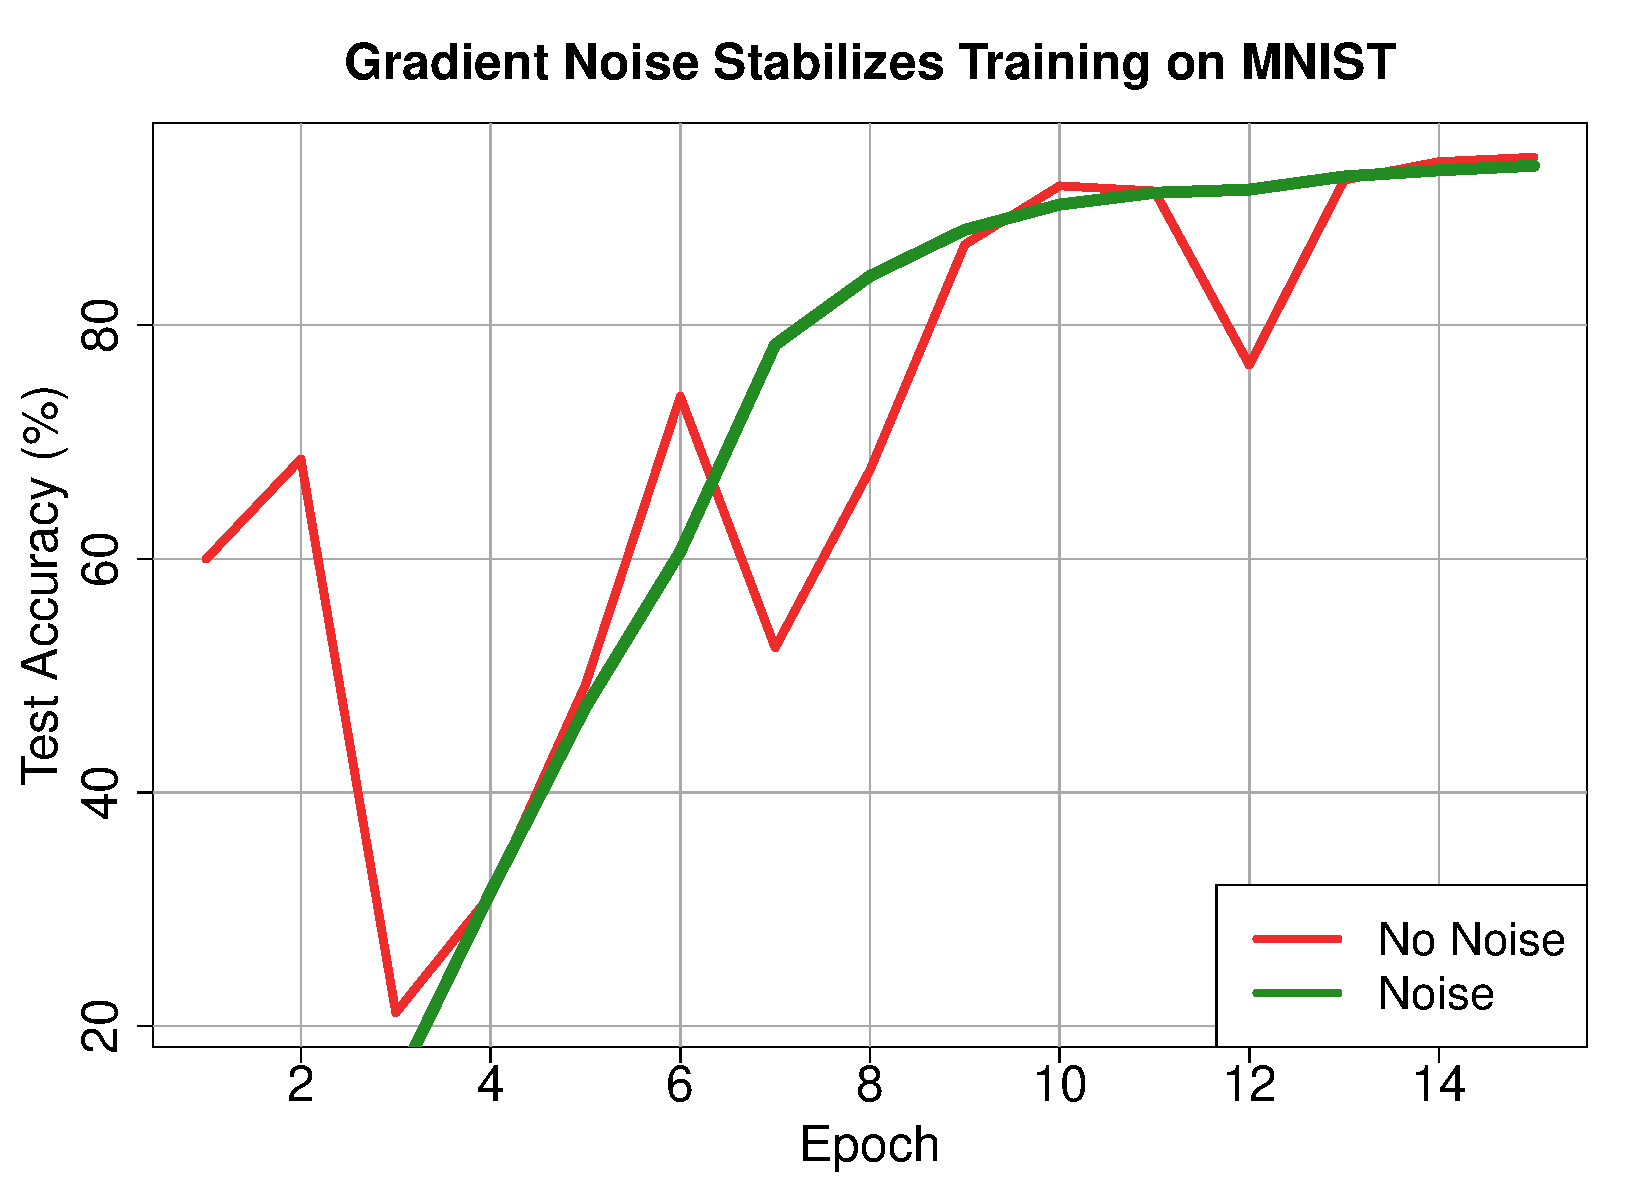
\includegraphics[width=0.6\textwidth]{mnistNoise.pdf}
\end{center}
\caption{Test accuracy for MNIST, with and without artificial gradient noise.}
\label{fig:mnist_stable}
\end{figure}


\subsection{CIFAR10}
We train the ResNet18 model (He et al 2015) on the CIFAR10 dataset (Krizhevsky 2009). 
The CIFAR10 dataset consists of 60,000 32x32 color images in 10 classes, with 50,000 training images and 10,000 test images.
We add gradient noise sampled from a standard normal distribution which is scaled by the schedule in Equation~\ref{eq:artificial_noise_scale} with $\eta = \{ 0.005, 0.01, 0.3 \}$.
We use SGD with momentum parameter set to $0.5$, and learning rates in a range from $0.01$ to $0.2$.
In our initial experiments we run the training for 20 epochs and record the final test accuracy.

The results for batch size up to 8,192 can be seen in Table~\ref{tab:cifar10_noise}.
Like in the MNIST experiments, the benefits of artificial noise manifest when the batch size gets sufficiently big.
The improvement in final test accuracy that artificial noise provides also increases as the batch size increases.

\begin{table}[h]
\begin{center}
\begin{tabular}{ c c c}
 Batch Size & Final Test Accuracy (\%) & Artificial Noise Final (\%) \\ 
 \hline
 1,024 & 86.36 & 84.88 \\
 2,048 & 84.54 & 84.16 \\
 4,096 & 79.33 & 82.28 \\  
 8,192 & 65.64 & 71.08 \\
\end{tabular}
\end{center}
\caption{CIFAR10 with Artificial Gradient Noise}
\label{tab:cifar10_noise}
\end{table}

[Still working on getting more results for CIFAR10]

%Unlike for the MNIST data set, we run into a memory limit when trying to load a batch size of 16,384 into memory onto our GPUs.
%In our pytorch implementation we develop a work-around by calling several {\tt forward()} and {\tt backward()} passes of the network before taking a step with SGD.
%This is not strictly equivalent to using a larger batch size because the batch normalization statistics will only be computed for the batch size that fits in memory.
%However our solution is still of interest because we wish to attain speedups from large batch parallelization, but do not want to be limited by the memory constraints of our particular setup.
%
%[Talk about experimental conditions, again] 
%
%\begin{table}[h]
%\label{tab:cifar10_simBatch}
%\begin{center}
%\begin{tabular}{ c c c}
% Batch Size & Final Test Accuracy (\%) & Artificial Noise Final (\%) \\ 
% \hline
% 16,384 & 57.42 & 60.98 \\
% 24,576 & 51.96 & 52.01 \\
%\end{tabular}
%\end{center}
%\caption{CIFAR10 with Artificial Gradient Noise and Simulated Large Batch}
%\end{table}

%\subsection{Penn TreeBank (?)}
%Choose one text data set or the other.
%
%\subsection{WikiText-2}
%Much of the literature on Large Batch SGD has focused on image recognition tasks using datasets.
%We perform language modeling experiments on the WikiText-2 dataset using a LSTM model.
%
%[Planning on running these experiments, have not yet]

\section{Full batch gradient descent with added noise}
We take Large Batch SGD to its logical conclusion by running full-batch gradient descent with added artificial noise.
The source of randomness of the stochastic gradient typically comes from the randomly sampled mini-batch.
However when the full batch is used to compute the gradient, there is no more randomness with respect to the empirical loss function.
This randomness in the gradients is important because it helps SGD to reach minima that generalize well.
We re-introduce randomness to the gradient with artificial noise as in Equation~\ref{eq:artificial_noise}.
This is essentially ``simulating" SGD.

It is uncertain if the noise which naturally occurs in the stochastic gradients has the same structure as Gaussian noise.
We conduct experiments on the MNIST data set, using the same network described in the previous section.
A learning rate of $0.01$ is used, with the noise scale schedule as in Equation~\ref{eq:artificial_noise_scale} with $\eta = 1$.
Both full batch gradient descent with and without additional noise are run for 100 epochs.
%\begin{table}[h]
%\label{tab:mnist_simSGD}
%\begin{center}
%\begin{tabular}{ c c c}
% Epochs & Test Accuracy GD (\%) & Simulated SGD (\%) \\ 
% \hline
% 25 & 61.51 & 76.67 \\
% 75 & 82.96 & 90.55 \\
% 500 & 96.10 & 97.13 \\
%\end{tabular}
%\end{center}
%\caption{MNIST with Simulated SGD}
%\end{table}
%We run the procedure for up to 500 epochs to allow the procedures to fully converge, and display the accuracy on test at several time slices in Table~\ref{tab:mnist_simSGD}.

\begin{figure}[t]
\begin{center}
  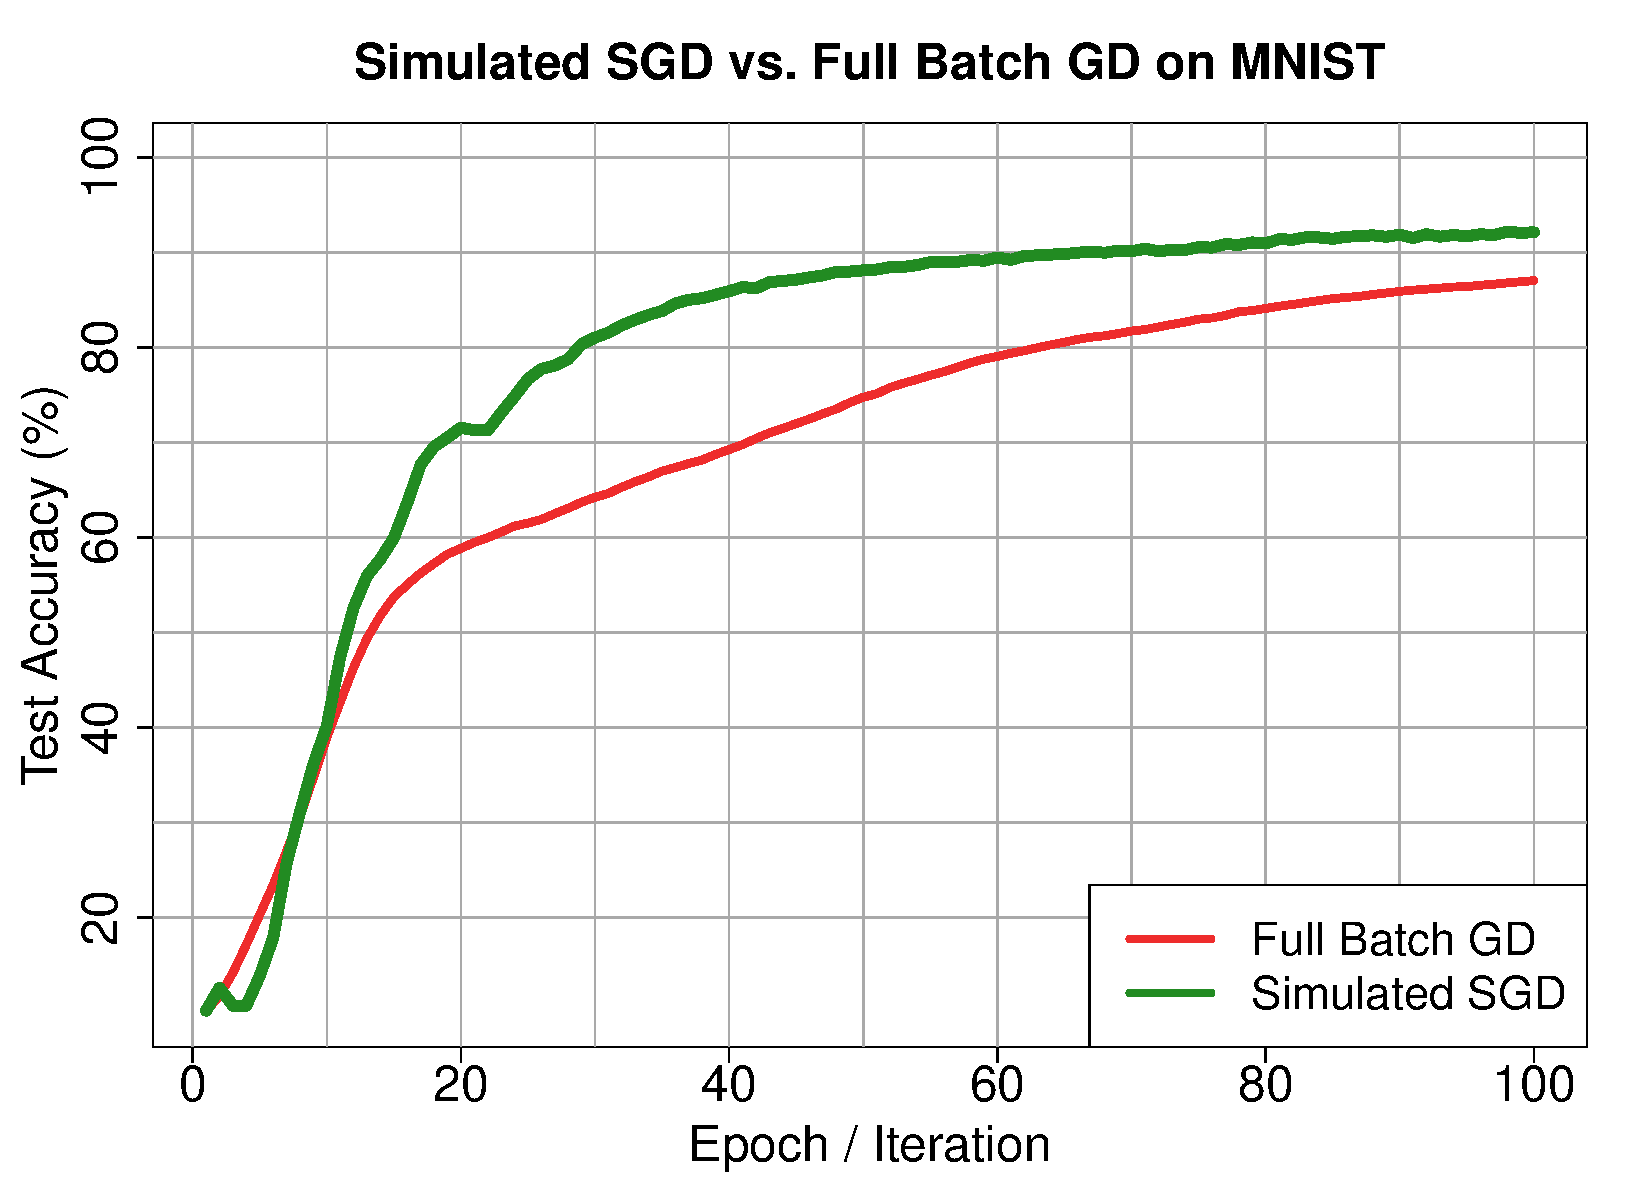
\includegraphics[width=0.6\textwidth]{mnistSimSGD.pdf}
\end{center}
\caption{Training full-batch gradient descent with and without artificial noise on MNIST.
By adding artificial noise to the full-batch gradient we are simulating SGD.
}
\label{fig:mnist_simSGD}
\end{figure}

We compare simulated SGD with regular full-batch gradient descent in Figure~\ref{fig:mnist_simSGD}. 
Adding noise to the true gradient significantly accelerates training over the full-batch gradient descent.
In addition the final achieved test accuracy is higher by 5\%.
We believe that the added noise helps the optimization procedure to more efficiently explore the non-convex loss landscape.
Because the full training set is used in each iteration, each epoch consists of exactly one iteration.
The simulated SGD procedure is able to converge in 100 iterations.

Because of the success of the simulated SGD procedure, Gaussian noise can be reasonable effective in simulating the natural noise in the stochastic gradients of SGD.
If the simulated SGD procedure is run for 500 epochs / iterations and allowed to converge, and the test accuracy is reported in Table~\ref{tab:mnist_simSGD}.
This accuracy is very close to the state-of-art results, which are just above 99\% depending on the network configuration~\url{http://yann.lecun.com/exdb/mnist/}.

\begin{table}[h]
\begin{center}
\begin{tabular}{ c c}
 Epochs & Simulated SGD Test Accuracy (\%) \\ 
 \hline
 %25 & 61.51 & 76.67 \\
 %75 & 82.96 & 90.55 \\
 500 & 97.13 \\
\end{tabular}
\end{center}
\caption{Test Accuracy for Converged Simulated SGD}
\label{tab:mnist_simSGD}
\end{table}
%We run the procedure for up to 500 epochs to allow the procedures to fully converge, and display the accuracy on test at several time slices in Table~\ref{tab:mnist_simSGD}.

It remains to be seen if state-of-the-art results can be achieved with simulated SGD by using different types of noise, potentially conditioned on the iterates (Zhu et al 2019).
Doing so would provide a convincing argument that the noise used to achieve such results would have a functional equivalent to the noise introduced through randomly sampled mini-batches.
%Because we are able to achieve test accuracy close to the state of the art values, this tells us that Gaussian noise is potentially a good approximation to the noise normally present in the stochastic gradients.


\section{Conclusion}
[Tentative]

We show that adding artificial noise to the gradient can improve the generalization performance of Large Batch SGD.
Additive noise can tune the signal-to-noise ratio of the stochastic gradients in a more careful way than scaling the learning rate.
We propose a simple to implement noise procedure, and present numerical experiments on image classification and language modeling tasks.
In addition, we take Large Batch SGD to its logical conclusion and show that SGD can be effectively simulated by performing full-batch gradient descent and adding artificial noise to the gradients.


% Story: Gradient noise stabilizes at the higher learning rates and higher batch sizes


%\subsection{Citations within the text}
%
%Citations within the text should be based on the \texttt{natbib} package
%and include the authors' last names and year (with the ``et~al.'' construct
%for more than two authors). When the authors or the publication are
%included in the sentence, the citation should not be in parenthesis (as
%in ``See \citet{Hinton06} for more information.''). Otherwise, the citation
%should be in parenthesis (as in ``Deep learning shows promise to make progress towards AI~\citep{Bengio+chapter2007}.'').
%
%The corresponding references are to be listed in alphabetical order of
%authors, in the \textsc{References} section. As to the format of the
%references themselves, any style is acceptable as long as it is used
%consistently.
%
%\subsection{Footnotes}
%
%Indicate footnotes with a number\footnote{Sample of the first footnote} in the
%text. Place the footnotes at the bottom of the page on which they appear.
%Precede the footnote with a horizontal rule of 2~inches
%(12~picas).\footnote{Sample of the second footnote}
%
%\subsection{Figures}
%
%All artwork must be neat, clean, and legible. Lines should be dark
%enough for purposes of reproduction; art work should not be
%hand-drawn. The figure number and caption always appear after the
%figure. Place one line space before the figure caption, and one line
%space after the figure. The figure caption is lower case (except for
%first word and proper nouns); figures are numbered consecutively.
%
%Make sure the figure caption does not get separated from the figure.
%Leave sufficient space to avoid splitting the figure and figure caption.
%
%You may use color figures.
%However, it is best for the
%figure captions and the paper body to make sense if the paper is printed
%either in black/white or in color.
%\begin{figure}[h]
%\begin{center}
%%\framebox[4.0in]{$\;$}
%\fbox{\rule[-.5cm]{0cm}{4cm} \rule[-.5cm]{4cm}{0cm}}
%\end{center}
%\caption{Sample figure caption.}
%\end{figure}
%
%\subsection{Tables}
%
%All tables must be centered, neat, clean and legible. Do not use hand-drawn
%tables. The table number and title always appear before the table. See
%Table~\ref{sample-table}.
%
%Place one line space before the table title, one line space after the table
%title, and one line space after the table. The table title must be lower case
%(except for first word and proper nouns); tables are numbered consecutively.
%
%\begin{table}[t]
%\caption{Sample table title}
%\label{sample-table}
%\begin{center}
%\begin{tabular}{ll}
%\multicolumn{1}{c}{\bf PART}  &\multicolumn{1}{c}{\bf DESCRIPTION}
%\\ \hline \\
%Dendrite         &Input terminal \\
%Axon             &Output terminal \\
%Soma             &Cell body (contains cell nucleus) \\
%\end{tabular}
%\end{center}
%\end{table}


\bibliography{iclr2019_conference}
\bibliographystyle{iclr2019_conference}

\end{document}
